\documentclass[paper=letter, fontsize=12pt]{scrartcl}

\usepackage[T1]{fontenc}
\usepackage[utf8]{inputenc}
\usepackage[english, spanish]{babel}
\usepackage{hyperref}
\usepackage{amsfonts,amsthm,amssymb}
\usepackage{amsmath}
\usepackage{listings}
\usepackage[dvipsnames]{xcolor}
\usepackage{sectsty}
\usepackage{dirtree}
\usepackage{booktabs}
\usepackage{enumitem}
\usepackage{graphicx}
\graphicspath{ {img/} }

\lstdefinestyle{mystyle}{
    backgroundcolor=\color{backcolour},
    commentstyle=\color{codegreen},
    keywordstyle=\color{magenta},
    numberstyle=\tiny\color{codegray},
    stringstyle=\color{codepurple},
    basicstyle=\footnotesize,
    breakatwhitespace=false,
    breaklines=true,
    captionpos=b,
    keepspaces=true,
    numbers=left,
    numbersep=5pt,
    showspaces=false,
    showstringspaces=false,
    showtabs=false,
    tabsize=2
}

\setlength{\DTbaselineskip}{20pt}
\DTsetlength{1em}{3em}{0.1em}{1pt}{4pt}

\allsectionsfont{\raggedright\large \textit\normalfont\scshape\emph}

\title{Práctica 3}

\subtitle{
  Lógica Computacional, 2018-2\\
  Facultad de Ciencias, UNAM
}

\author{
  \normalsize
  Noé Salomón Hernández Sánchez\\
  \normalsize
  \texttt{\href{mailto:no.hernan@gmail.com}{no.hernan@gmail.com}}
  \and
  \normalsize
  María del Carmen Sánchez Almanza\\
  \normalsize
  \texttt{\href{mailto:carmensanchez@ciencias.unam.mx}{carmensanchez@ciencias.unam.mx}}
  \and
  \normalsize
  Albert Manuel Orozco Camacho\\
  \normalsize
  \texttt{\href{mailto:alorozco53@ciencias.unam.mx}{alorozco53@ciencias.unam.mx}}
}

\date{\today}

\begin{document}

\maketitle

\section{Objetivo}

\noindent
Los asistentes automáticos de demostraciones nos brindan un paradigma especial\
de lo que implica escribir una prueba formal: en cada momento nos planteamos un\
objetivo al que hemos de llegar mediante argumentos bien fundamentados. Para este\
curso, el algoritmo de verificación de fórmulas derivado de las reglas de deducción\
natural motivan al uso de una herramienta como \verb+Coq+.\par
Mediante el asistente de pruebas francés exploraremos otro de los métodos de\
resolución del problema de satisfacibilidad, cuya eficiencia depende de la destreza\
del programador entorno a su uso. A pesar de que restringiremos el uso de \verb+Coq+\
a fórmulas de los cálculos vistos en el curso, es importante notar y destacar su uso\
para tareas como \emph{verificación de software} y \emph{razonamiento automatizado},\
las cuales están adquiriendo mayor preponderancia en el mundo computacional moderno.

\section{Ejercicios}

\noindent
El esqueleto de código de la práctica se encuentra en \url{https://github.com/alorozco53/LabLogComp-2018-2/tree/pract3/src}.\
Asegúrese de haber instalado \verb+CoqIDE+ o \verb+ProofGeneral+ en su computadora,\
mediante el \href{https://github.com/alorozco53/LabLogComp-2018-2/blob/master/notas/session9/coq.md}{\underline{tutorial presentado en clase}}.

\subsection{Correctud de fórmulas}

\noindent
Para las siguientes fórmulas, dé una demostración basada en tácticas de Coq.

\begin{enumerate}
\item $p \to q, q \to r \vee s, \neg s, p \vdash r$.
\item $\vdash (p \to q) \to (p \vee r \to q \vee r)$. \emph{Consejo}: dé una demostración\
  \emph{por reducción al absurdo} mediante el uso de una doble negación del consecuente de la fórmula.\
  Es decir, recuerde que para toda fórmula $A$ y $B$,
  \[A \to B \equiv A \to \neg \neg B.\]
\item
  \begin{equation*}
    \begin{aligned}
      &\exists x Q(x)\\
      &\forall x (Q(x) \wedge \exists y P(y) \to Q(f(x)))\\
      &\forall z (Q(z) \to Q(g(z)))\\
      \midrule
      &\therefore P(b) \to \exists w Q(f(g(w)))
    \end{aligned}
  \end{equation*}
  Recuerde que se debe de definir un universo de discurso (\verb+D+) y que los predicados se modelan\
  mediante un tipo que toma cuantos valores indique su aridad para ``devolver'' algo de tipo \verb+Prop+.\
  Por ejemplo, el predicado $P$ tendría tipo \verb+D -> Prop+. Asímismo, no olvide definir la constante\
  $b$ como \verb+Variable+ de tipo \verb+D+ y las variables $f$ y $g$ ambas como \verb+Variable+ de tipo\
  \verb+D -> D+.
\item
  \begin{equation*}
    \begin{aligned}
      &\exists x (\neg P(x) \vee Q(x))\\
      \midrule
      &\therefore \exists x \neg (P(x) \wedge \neg Q(x))
    \end{aligned}
  \end{equation*}
\item
  \begin{equation*}
    \begin{aligned}
      &\forall x (P(x) \to Q(x))\\
      &\forall y (R(b) \vee Q(y) \to S(a))\\
      \midrule
      &\therefore \forall z (P(z) \to \exists y S(y))
    \end{aligned}
  \end{equation*}
\end{enumerate}

\subsection{Traducción y verificación}

\noindent
Demostrar la correctud de los siguientes argumentos.

\begin{enumerate}[resume]
\item Usando exclusivamente la signatura $\{F^{(1)}, V^{(1)}, B^{(1)}, E^{(1)}, P^{(1)}, L^{(1)}, S^{(1)}, C^{(2)}\}$\
  con significados \textit{ser feliz, ser vampiro, ser bruja, emborracharse, pernoctar en cementerio,}
  \textit{violar la ley, ser sepulturero, convivir}, respectivamente, demostrar usando tácticas que:
  \begin{center}
    \textit{
      Un vampiro sólo es feliz si se emborracha o pernocta en un cementerio. Quien pernocta en un
      cementerio viola la ley o es sepulturero. Una bruja sólo es feliz si convive con un vampiro feliz,
      que no se emborracha y que no viola la ley. Hay brujas felices. Por lo tanto algunos vampiros
      son sepultureros.
    }
  \end{center}
\item Harry Potter estaba teniendo dificultades para resolver una pista en la penúltima\
  prueba del Torneo de los Tres Magos. La prueba consiste en revisar la validez del argumento\
  siguiente:
    \begin{center}
      \textit{
        El Patronum lo hizo Snape o, hay que jugar Quidditch y molestar a Ron. Si el
        Patronum lo hizo Snape, hay que jugar Quidditch. Hay que jugar Quidditch si y sólo si
        Slytherin es la mejor casa de Hogwarts. Por lo tanto, hay que jugar Quidditch y Slytherin
        es la mejor casa de Hogwarts.
      }
    \end{center}
    Ayude a Harry Potter a pasar a la siguiente fase, dándole una serie de tácticas de \verb+Coq+\
    que verifiquen su argumento.
\end{enumerate}

\subsection{Un agente racional}

\begin{figure}[h]
  \centering
  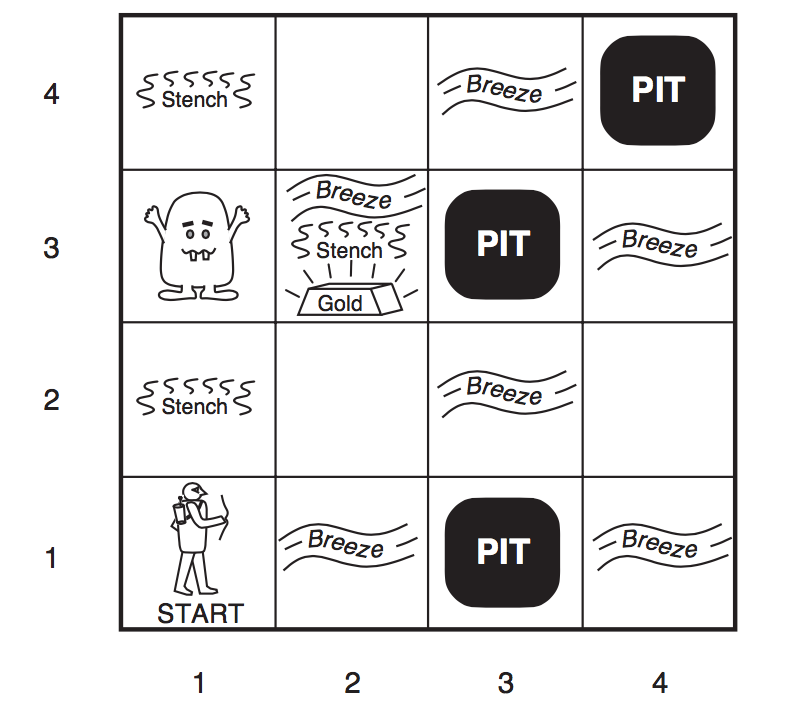
\includegraphics[width=0.5\textwidth]{wumpusworld}
  \caption[CAPTION WUMPUS]{
    El tablero del \emph{mundo de wumpus}. El agente, inicialmente, se encuentra en la
    casilla \texttt{[1,1]} y debe de averiguar la mejor estrategia que le conduzca al
    bloque de oro (casilla \texttt{[2,3]}) sin entrar en contacto con el monstruo y
    sin caer en un pozo (\emph{PIT}). Tomado de \footnotemark.
  }
  \label{wumpusfig}
\end{figure}
\footnotetext{\url{http://www.cs.uku.fi/~mnykanen/TEK/teklectures6.pdf}}

\noindent
En el mundo de \emph{wumpus} (término inglés para referirse a una especie de monstruo)\
un jugador debe de explorar un camino lleno de peligros con el fin de encontrar\
el bloque de oro que le dé la victoria. El juego presentado en este apartado es\
(casi) equivalente al utilizado dentro del libro \emph{Artificial Intelligence: A Modern Approach}%
\footnote{\url{http://aima.cs.berkeley.edu}}.\par
El mundo de \emph{wumpus} consta de una cuadrícula; el jugador inicialmente comienza su aventura\
en una de las esquinas y su objetivo es regresar a su posición inicial con el bloque de oro en\
su haber. El personaje únicamente se puede mover horizontal y verticalmente en un entorno\
que contiene algunas casillas que le harían perdedor automáticamente de entrar en ellas:
\begin{itemize}
\item hay un \textbf{monstruo} hediondo, el cual es capaz de comerse vivo al personaje y
\item existen varias casillas con \textbf{pozos} (\emph{PIT}), los cuales pueden succionar al protagonista\
  al más allá.
\end{itemize}\par
Afortunadamente existen algunas pistas que le permitirán al jugador esquivar las casillas peligrosas\
para sí mismo. Si el jugador se encuentra en la casilla \verb+[i,j]+ (donde \verb+i+ indica la posición\
horizontal de izquierda a derecha y \verb+j+ indica la posición vertical de abajo hacia arriba),\
entonces éste puede identificar la existencia del monstruo o de un pozo en una casilla adyacente:
\begin{itemize}
\item El fuerte olor del monstruo, despide un hedor (\emph{STENCH}) que se percibe\
  en las casillas vertical y horizontalmente adyacentes.
\item El poder succionador de un pozo, ocasiona que se sienta una brisa (\emph{BREEZE})\
  en las casillas vertical y horizontalmente adyacentes.
\end{itemize}\par
Habiendo establecido lo anterior, modelamos el mundo de \emph{wumpus} mediante las siguientes\
variables proposicionales:
\begin{itemize}
\item $P_{i,j}$ \emph{si y sólo si} hay un pozo en la casilla \verb+[i,j]+;
\item $W_{i,j}$ \emph{si y sólo si} está el monstruo en la casilla \verb+[i,j]+;
\item $B_{i,j}$ \emph{si y sólo si} se siente una brisa en la casilla \verb+[i,j]+;
\item $S_{i,j}$ \emph{si y sólo si} se percibe mal olor en la casilla \verb+[i,j]+.
\end{itemize}\par
De las anteriores definiciones, de pueden (¡y deben!) deducir algunas equivalencias dadas las pistas,\
de percepción que posee el jugador. Por ejemplo la sensación de brisa en la casilla \verb+[i,j]+\
equivale a la existencia de un pozo en alguna de las casillas \verb_[i+1,j]_, \verb_[i,j+1]_,\
\verb_[i-1,j]_ ó \verb_[i,j-1]_, a saber,
\begin{equation}
  B_{i,j} \leftrightarrow (P_{i+1,j} \vee P_{i,j+1} \vee P_{i-1,j} \vee P_{i,j-1}).\label{pot-breeze-equiv}
\end{equation}\par
Para la implementación en \verb+Coq+, definimos las variables anteriormente establecidas, mediante tipos\
que toman dos números naturales y devuelven el tipo \verb+Prop+. Por ejemplo, $S_{i,j}$ se definiría con el\
enunciado:
\begin{verbatim}
Variable S : nat -> nat -> Prop.
\end{verbatim}\par
Obsérvese que estamos trabajando únicamente con lógica proposicional. En \verb+Coq+, decir que hay un pozo en\
la casilla \verb+[3,5]+ se expresa mediante \verb+P 3 5+. De esta manera, cualquier expresión que posea los\
dos números que indican la posición de las casillas es, en sí, una variable proposicional; por ejemplo,\
se puede demostrar el siguiente teorema trivial:
\begin{verbatim}
((P 1 1 -> W 4 6) /\ P 1 1) -> W 4 6.
\end{verbatim}\par
Supongamos que el jugador desarrolla su partida como en la cuadrícula de la Figura \ref{wumpusfig}.\
Inicialmente, no hay ni pozo ni monstruo en la casilla inicial:
\begin{enumerate}[label=H\arabic*]
\item $\neg P_{1,1} \wedge \neg W_{1,1}$.
\end{enumerate}\par
Más aún, supongamos que el jugador ya ha visitado las casillas \verb+[1,2]+ y \verb+[2,1]+, por lo que\
es conocimimento del jugador las siguientes equivalencias, del estilo de la Ecuación \ref{pot-breeze-equiv}:
\begin{enumerate}[label=H\arabic*, resume]
\item $B_{1,1} \leftrightarrow (P_{2,1} \vee P_{1,2})$,
\item $S_{1,1} \leftrightarrow (W_{2,1} \vee W_{1,2})$,
\item $B_{2,1} \leftrightarrow (P_{1,1} \vee P_{2,2} \vee P_{3,1})$,
\item $S_{1,2} \leftrightarrow (W_{1,1} \vee W_{2,2} \vee W_{1,3})$.
\end{enumerate}\par
Además, se tiene como hecho lo siguiente:
\begin{enumerate}[label=H\arabic*, resume]
\item $\neg B_{1,1}$,
\item $\neg S_{1,1}$,
\item $\neg B_{1,2}$,
\item $\neg S_{2,1}$,
\item $S_{1,2}$,
\item $B_{2,1}$.
\end{enumerate}
Queremos, entonces, ayudarle al jugador a decidir correctamente que la casilla \verb+[2,2]+ es\
una opción segura para continuar con su trayecto. Para ello, necesitamos mostrar\
formalmente que $\neg P_{2,2} \wedge \neg W_{2,2}$. Para finalizar con la implementación en\
\verb+Coq+, se recomienda asumir las hipótesis (H1 - H11) previamente presentadas mediante\
enunciados \verb+Definition+. Por ejemplo,
\begin{verbatim}
Definition H2 : B 1 1 <-> (P 2 1 \/ P 1 2).
\end{verbatim}\par
Se recomienda realizar la solución de este problema en un archivo aparte de los demás de la práctica.

\section{Entrega}

\noindent
La fecha de entrega es el próximo \textbf{viernes 11 de mayo de 2018} por la plataforma\
de \emph{Google Classroom} del curso y siguiendo los lineamientos del laboratorio.

\end{document}
